\chapterold{"Прикуп" в игре "Марьяж"}

\epigraph{Знал бы прикуп --- жил бы в Сочи.}{Поговорка.}

"Марьяж" --- старая и довольно популярная версия игры в "Преферанс" под DOS.

Играют три игрока, каждому раздается по 10 карт, остальные 2 остается в т.н. "прикупе".
Начинаются торги, во время которых "прикуп" скрыт.
Он открывается после того, как один из игроков сделает "заказ".

Знание карт в "прикупе" обычно имеет решающее преимущество.

Вот так в игре выглядит состояние "торгов", и "прикуп" посредине, скрытый:

\begin{figure}[H]
\centering
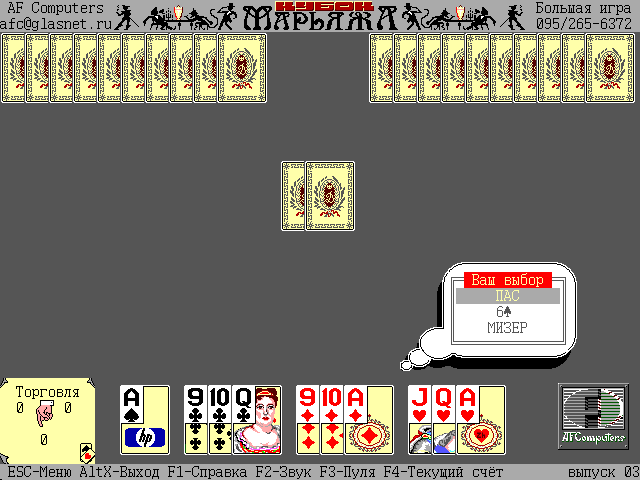
\includegraphics[scale=\FigScale]{examples/marriage/initial_not_patched.png}
\caption{"Торги"}
\end{figure}

Попробуем "подсмотреть" карты в "прикупе" в этой игре.

Для начала --- что мы знаем?
Игра под DOS, датируется 1997-м годом. IDA показывает имена стандартных функций вроде 
\TT{@GetImage\$q7Integert1t1t1m3Any} --- это "манглинг" типичный для Borland Pascal, что позволяет сделать вывод,
что сама игра написана на Паскале и скомпилирована Borland Pascal-ем.

Файлов около 10-и и некоторые имеют текстовую строку в заголовке "Marriage Image Library" --- вероятно,
это библиотеки спрайтов.

В IDA можно увидеть что используется функция \TT{@PutImage\$q7Integert1m3Any4Word}, которая, собственно,
рисует некий спрайт на экране.
Она вызывается по крайней мере из 8-и мест.
Чтобы узнать что происходит в каждом из этих 8-и мест, мы можем блокировать работу каждой функции и смотреть,
что будет происходить.
Например, первая ф-ция имеет адрес seg002:062E, и она заканчивается инструкцией \INS{retf 0Eh} на seg002:102A.
Это означает что метод вызовов ф-ций в Borland Pascal под DOS схож с stdcall --- вызываемая ф-ция должна сама
возвращать стек в состояние до того как началась передача аргументов.
В самом начале этой ф-ции вписываем инструкцию "retf 0eh", либо 3 байта: \TT{CA 0E 00}.
Запускаем "Марьяж" и внешне вроде бы ничего не изменилось.

Переходим ко второй ф-ции, которая активно использует \TT{@PutImage\$q7Integert1m3Any4Word}.
Она находится по адресу seg008:0AB5 и заканчивается инструкцией \INS{retf 0Ah}.
Вписываем эту инструкцию в самом начале и запускаем:

\begin{figure}[H]
\centering
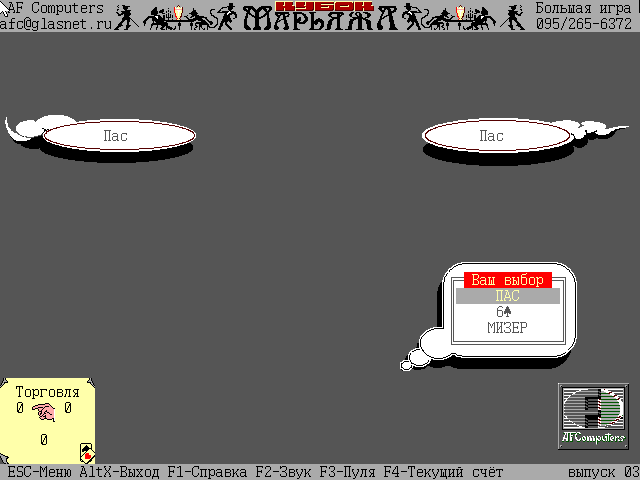
\includegraphics[scale=\FigScale]{examples/marriage/draw_card_bypass.png}
\caption{Карт нет}
\end{figure}

Карт не видно вообще. И видимо, эта функция их отображает, мы её заблокировали, и теперь карт не видно.
Назовем эту ф-цию в IDA \TT{draw\_card()}.
Помимо \TT{@PutImage\$q7Integert1m3Any4Word}, в этой ф-ции вызываются также ф-ции @SetColor\$q4Word, 
\TT{@SetFillStyle\$q4Wordt1}, \TT{@Bar\$q7Integert1t1t1}, \TT{@OutTextXY\$q7Integert16String}.

Сама ф-ция \TT{draw\_cards()} (её название мы дали ей сами только что) вызывается из 4-х мест.
Попробуем точно также "блокировать" каждую ф-цию.

Когда я "блокирую" вторую, по адресу seg008:0DF3 и запускаю программу, вижу такое:

\begin{figure}[H]
\centering
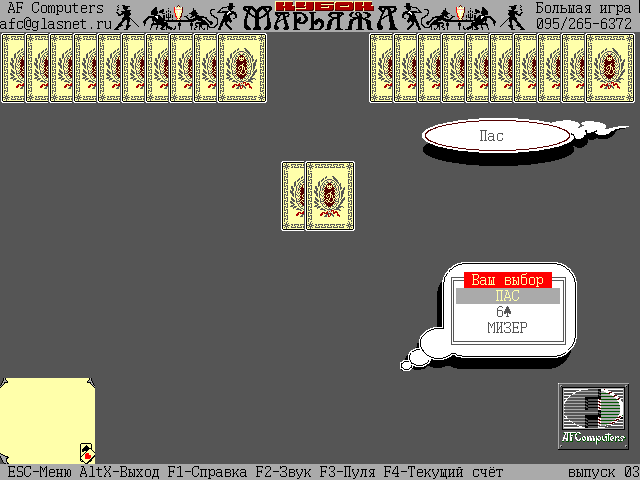
\includegraphics[scale=\FigScale]{examples/marriage/draw_players_cards.png}
\caption{Все карты кроме карт игрока}
\end{figure}

Видны все карты, кроме карт игрока. Видимо, эта функция рисует карты игрока. \\
Я переименовываю её в IDA в \TT{draw\_players\_cards()}.

Четвертая ф-ция, вызывающая \TT{draw\_cards()}, находится по адресу seg008:16B3, и когда я её "блокирую",
я вижу в игре такое:

\begin{figure}[H]
\centering
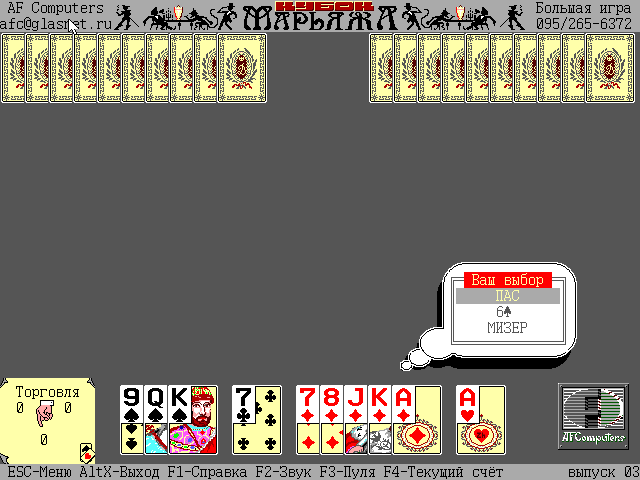
\includegraphics[scale=\FigScale]{examples/marriage/no_prikup.png}
\caption{"Прикупа" нет}
\end{figure}

Все карты есть, кроме "прикупа". Более того, эта ф-ция вызывает только \TT{draw\_cards()}, и только 2 раза.
Видимо эта ф-ция и отображает карты "прикупа".
Будем рассматривать её внимательнее.

\begin{lstlisting}
seg008:16B3 draw_prikup     proc far                ; CODE XREF: seg010:00B0
seg008:16B3                                         ; sub_15098+6
seg008:16B3
seg008:16B3 var_E           = word ptr -0Eh
seg008:16B3 var_C           = word ptr -0Ch
seg008:16B3 arg_0           = byte ptr  6
seg008:16B3
seg008:16B3                 enter   0Eh, 0
seg008:16B7                 mov     al, byte_2C0EA
seg008:16BA                 xor     ah, ah
seg008:16BC                 imul    ax, 23h
seg008:16BF                 mov     [bp+var_C], ax
seg008:16C2                 mov     al, byte_2C0EB
seg008:16C5                 xor     ah, ah
seg008:16C7                 imul    ax, 0Ah
seg008:16CA                 mov     [bp+var_E], ax
seg008:16CD                 cmp     [bp+arg_0], 0
seg008:16D1                 jnz     short loc_1334A
seg008:16D3                 cmp     byte_2BB08, 0
seg008:16D8                 jz      short loc_13356
seg008:16DA
seg008:16DA loc_1334A:                              ; CODE XREF: draw_prikup+1E
seg008:16DA                 mov     al, byte ptr word_32084
seg008:16DD                 mov     byte_293AD, al
seg008:16E0                 mov     al, byte ptr word_32086
seg008:16E3                 mov     byte_293AC, al
seg008:16E6
seg008:16E6 loc_13356:                              ; CODE XREF: draw_prikup+25
seg008:16E6                 mov     al, byte_293AC
seg008:16E9                 xor     ah, ah
seg008:16EB                 push    ax
seg008:16EC                 mov     al, byte_293AD
seg008:16EF                 xor     ah, ah
seg008:16F1                 push    ax
seg008:16F2                 push    [bp+var_C]
seg008:16F5                 push    [bp+var_E]
seg008:16F8                 cmp     [bp+arg_0], 0
seg008:16FC                 jnz     short loc_13379
seg008:16FE                 cmp     byte_2BB08, 0
seg008:1703                 jnz     short loc_13379
seg008:1705                 mov     al, 0
seg008:1707                 jmp     short loc_1337B
seg008:1709 ; ---------------------------------------------------------------------------
seg008:1709
seg008:1709 loc_13379:                              ; CODE XREF: draw_prikup+49
seg008:1709                                         ; draw_prikup+50
seg008:1709                 mov     al, 1
seg008:170B
seg008:170B loc_1337B:                              ; CODE XREF: draw_prikup+54
seg008:170B                 push    ax
seg008:170C                 push    cs
seg008:170D                 call    near ptr draw_card
seg008:1710                 mov     al, byte_2C0EA
seg008:1713                 xor     ah, ah
seg008:1715                 mov     si, ax
seg008:1717                 shl     ax, 1
seg008:1719                 add     ax, si
seg008:171B                 add     ax, [bp+var_C]
seg008:171E                 mov     [bp+var_C], ax
seg008:1721                 cmp     [bp+arg_0], 0
seg008:1725                 jnz     short loc_1339E
seg008:1727                 cmp     byte_2BB08, 0
seg008:172C                 jz      short loc_133AA
seg008:172E
seg008:172E loc_1339E:                              ; CODE XREF: draw_prikup+72
seg008:172E                 mov     al, byte ptr word_32088
seg008:1731                 mov     byte_293AD, al
seg008:1734                 mov     al, byte ptr word_3208A
seg008:1737                 mov     byte_293AC, al
seg008:173A
seg008:173A loc_133AA:                              ; CODE XREF: draw_prikup+79
seg008:173A                 mov     al, byte_293AC
seg008:173D                 xor     ah, ah
seg008:173F                 push    ax
seg008:1740                 mov     al, byte_293AD
seg008:1743                 xor     ah, ah
seg008:1745                 push    ax
seg008:1746                 push    [bp+var_C]
seg008:1749                 push    [bp+var_E]
seg008:174C                 cmp     [bp+arg_0], 0
seg008:1750                 jnz     short loc_133CD
seg008:1752                 cmp     byte_2BB08, 0
seg008:1757                 jnz     short loc_133CD
seg008:1759                 mov     al, 0
seg008:175B                 jmp     short loc_133CF
seg008:175D ; ---------------------------------------------------------------------------
seg008:175D
seg008:175D loc_133CD:                              ; CODE XREF: draw_prikup+9D
seg008:175D                                         ; draw_prikup+A4
seg008:175D                 mov     al, 1
seg008:175F
seg008:175F loc_133CF:                              ; CODE XREF: draw_prikup+A8
seg008:175F                 push    ax
seg008:1760                 push    cs
seg008:1761                 call    near ptr draw_card ; prikup #2
seg008:1764                 leave
seg008:1765                 retf    2
seg008:1765 draw_prikup     endp
\end{lstlisting}

Интересно посмотреть, как именно вызывается \TT{draw\_prikup()}. У нее только один аргумент.

Иногда она вызывается с аргументом 1:

\begin{lstlisting}
...
seg010:084C                 push    1
seg010:084E                 call    draw_prikup
...
\end{lstlisting}

А иногда с аргументом 0, причем вот в таком контексте, где уже есть другая знакомая функция:

\begin{lstlisting}
seg010:0067                 push    1
seg010:0069                 mov     al, byte_31F41
seg010:006C                 push    ax
seg010:006D                 call    sub_12FDC
seg010:0072                 push    1
seg010:0074                 mov     al, byte_31F41
seg010:0077                 push    ax
seg010:0078                 call    draw_players_cards
seg010:007D                 push    2
seg010:007F                 mov     al, byte_31F42
seg010:0082                 push    ax
seg010:0083                 call    sub_12FDC
seg010:0088                 push    2
seg010:008A                 mov     al, byte_31F42
seg010:008D                 push    ax
seg010:008E                 call    draw_players_cards
seg010:0093                 push    3
seg010:0095                 mov     al, byte_31F43
seg010:0098                 push    ax
seg010:0099                 call    sub_12FDC
seg010:009E                 push    3
seg010:00A0                 mov     al, byte_31F43
seg010:00A3                 push    ax
seg010:00A4                 call    draw_players_cards
seg010:00A9                 call    sub_1257A
seg010:00AE                 push    0
seg010:00B0                 call    draw_prikup
seg010:00B5                 mov     byte_2BB95, 0
\end{lstlisting}

Так что единственный аргумент у \TT{draw\_prikup()} может быть или 0 или 1, т.е., это, возможно, булевый тип.
На что он влияет внутри самой ф-ции?
При ближайшем рассмотрении видно, что входящий 0 или 1 передается в \TT{draw\_card()}, т.е., у последней тоже есть
булевый аргумент.
Помимо всего прочего, если передается 1, то по адресам seg008:16DA и seg008:172E копируются несколько байт
из одной группы глобальных переменных в другую.

Эксперимент: здесь 4 раза сравнивается единственный аргумент с 0 и далее следует \INS{JNZ}.
Что если сравнение будет происходит с 1, и, таким образом, работа функции \TT{draw\_prikup()} будет обратной?
Патчим и запускаем:

\begin{figure}[H]
\centering
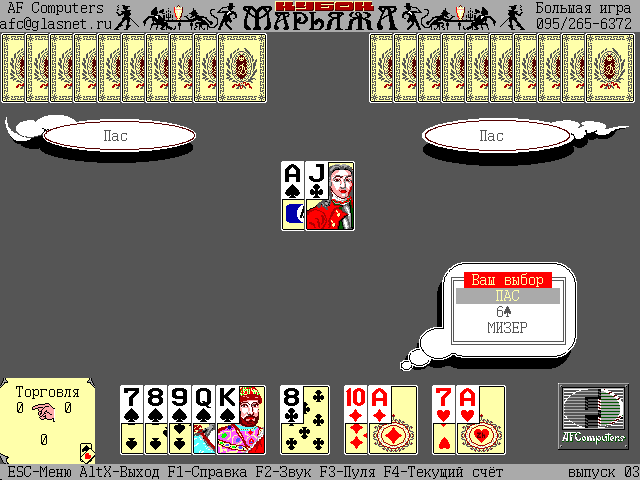
\includegraphics[scale=\FigScale]{examples/marriage/patch1.png}
\caption{"Прикуп" открыт}
\end{figure}

"Прикуп" открыт, но когда я делаю "заказ", и, по логике вещей, "прикуп" теперь должен стать открытым,
он наоборот становится закрытым:

\begin{figure}[H]
\centering
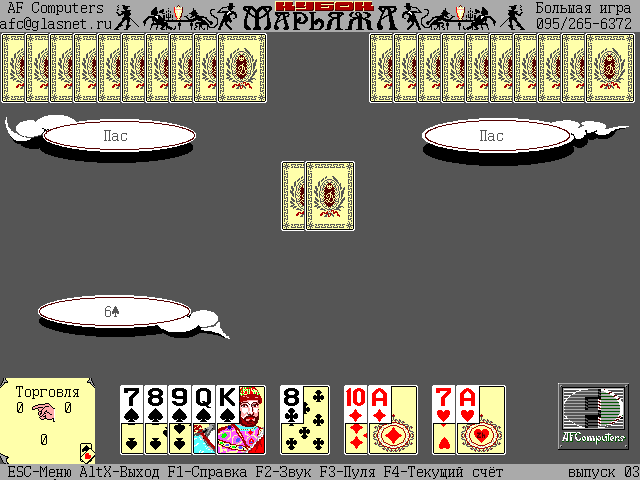
\includegraphics[scale=\FigScale]{examples/marriage/patch2.png}
\caption{"Прикуп" закрыт}
\end{figure}

Всё ясно: если аргумент \TT{draw\_prikup()} нулевой, то карты рисуются рубашкой вверх, если 1, то открытые.
Этот же аргумент передается в \TT{draw\_card()} --- эта ф-ция может рисовать и открытые и закрытые карты.

Пропатчить "Марьяж" теперь легко, достаточно исправить все условные переходы так, как будто бы в ф-цию
всегда приходит 1 в аргументе и тогда "прикуп" всегда будет открыт.

Но что за байты копируются в seg008:16DA и seg008:172E?
Я попробовал забить инструкции копирования \MOV \NOP{}-ами --- "прикуп" вообще перестал отображаться.

Тогда я сделал так, чтобы всегда записывалась 1:

\begin{lstlisting}
...
00004B5A: B001                           mov         al,1
00004B5C: 90                             nop
00004B5D: A26D08                         mov         [0086D],al
00004B60: B001                           mov         al,1
00004B62: 90                             nop
00004B63: A26C08                         mov         [0086C],al
...
\end{lstlisting}

Тогда "прикуп" отображается как два пиковых туза.
А если первый байт --- 2, а второй --- 1, получается трефовый туз.
Видимо так и кодируется масть карты, а затем и сама карта.
% TODO \ref{} сюда о том, как можно передавать аргументы в глоб.переменных
А \TT{draw\_card()} затем считывает эту информацию из пары глобальных переменных.
А копируется она тоже из глобальных переменных, где собственно и находится состояние карт у игроков и в прикупе
после случайной тасовки.
Но нельзя забывать что если мы сделаем так, что в "прикупе" всегда будет 2 пиковых туза, это будет только
на экране так отображаться, а в памяти состояние карт останется таким же, как и после тасовки.

Всё понятно: автор решил сделать одну ф-цию для отрисовки и закрытого и открытого прикупа, поэтому нам, можно сказать,
повезло.
Могло быть труднее: в самом начале рисовались бы просто две рубашки карт, а открытый прикуп только потом.

Я также пробовал сделать шутку-пранк: во время торгов одна карта "прикупа" открыта, а вторая закрыта, а после "заказа",
наоборот, первая закрыта, а вторая открывается. В качестве упражнения, вы можете попробовать сделать так.

Еще кое-что: чтобы сделать прикуп открытым, ведь можно же найти место где вызывается \TT{draw\_prikup()} и поменять 0
на 1. Можно, только это место не в головой marriage.exe, а в marriage.000, а это DOS-овский оверлей (начинается
с сигнатуры "FBOV").

В качестве упражнения, можно попробовать подсматривать состояние всех карт, и у обоих игроков.
Для этого нужно отладчиком смотреть состояние глобальной памяти рядом с тем, откуда считываются обе карты
прикупа.

Файлы: \\
оригинальная версия: \url{http://beginners.re/examples/marriage/original.zip}, \\
пропатченная мною версия: \url{http://beginners.re/examples/marriage/patched.zip} 
(все 4 условных перехода после \TT{cmp [bp+arg\_0], 0} заменены на \JMP).

